\section{Description de la fen�tre principale}

\begin{figure}[!htpb]
  \begin{center}
   	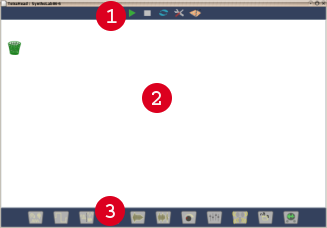
\includegraphics{images/screenshot.png}
    \caption{Capture d'�cran de la fen�tre principale}
  \end{center}
\end{figure}

Elle compte trois zones :
\begin{enumerate}
\item Une barre d'outils de commandes, situ�e en haut de la fen�tre
\item Une zone centrale de travail
\item Une barre d'outils de cr�ation de modules, en bas de la fen�tre
\end{enumerate}

paf le chien

\subsection{La barre d'outils de commande}

Avec cette barre d'outils, vous pourrez lancer (ou arr�ter)
l'ex�cution du syntht�tiseur. Elle comporte trois boutons :
\begin{itemize}
\item Un bouton \emph{Lecture} : En cliquant sur ce bouton, vous
d�marrerez l'ex�cution du synth�tiseur.
\item Un bouton \emph{Arr�t} : Un clic sur ce bouton stoppe
l'ex�cution du synth�tiseur.
\item Un bouton \emph{Reset} : 
\end{itemize}

%\subsection{}
%\subsection{}






















